\documentclass[12pt]{article}
\usepackage[spanish,es-tabla]{babel}
\usepackage{natbib}
\usepackage{url}
\usepackage{float}
\usepackage[utf8]{inputenc}
\usepackage{amsmath}
\usepackage{graphicx}
\usepackage{fancyhdr}
\usepackage{longtable}
\usepackage{vmargin}
\usepackage{listings}
\usepackage{hyperref}
\usepackage{multirow}
\usepackage{xcolor}
\usepackage{caption}
\usepackage{subcaption}

\setmarginsrb{3 cm}{2.5 cm}{3 cm}{2.5 cm}{1 cm}{1.5 cm}{1 cm}{1.5 cm}

\title{Proyecto final}
\date{\today}

\makeatletter
\let\thetitle\@title
\let\theauthor\@author
\let\thedate\@date
\makeatother

\pagestyle{fancy}
\fancyhf{}
\rhead{\theauthor}
\lhead{\thetitle}
\cfoot{\thepage}

\addto\captionsspanish{
  \renewcommand{\contentsname}%
    {Tabla de contenido}%
}

\begin{document}
    \pagestyle{fancy}
    \fancyhf{}

    \lhead{\begin{picture}(0,0) \put(0,0){
\includegraphics[width=30mm]{images/Logo2.png}} \end{picture}}
    \renewcommand{\headrulewidth}{0.7pt}
    \fancyhead[R]{Proyecto final}
\fancyfoot[R]{\thepage}

\begin{titlepage}
	\centering
    
\includegraphics[scale = 0.45]{images/Logo.png}\\[0.5 cm]	% University Logo
    \textsc{\large Universidad de los Andes\\
        \vspace{0.2cm} 
        Facultad de Ingeniería\\
        \vspace{0.3cm} 
        Proyecto final}\\[2.0 cm]	% University Name
	\textsc{\Large Procesamiento de lenguaje natural}\\[0.5 cm]
	% Course Code
	\rule{\linewidth}{0.2 mm} \\[0.4 cm]
	{ \LARGE \bfseries \thetitle}\\
	\rule{\linewidth}{0.2 mm} \\[1.5 cm]
	
	\large
			\emph{Presentado por:} \\
			Juan David García Hernández\\
			Nicolás Rocha Pacheco\\
			César Daniel Garrido Urbano\\
			
	\vfill
	\large
			\emph{Presentado a:}\\
			Rubén Francisco Manrique Pirmanrique\\
\end{titlepage}

\thispagestyle{empty}
\tableofcontents
\pagebreak

\setcounter{page}{1}
\section{Introducción}
\section{Introducción}

La reciente crisis mundial ocasionada por la pandemia del COVID-19 ha dado mucho de que hablar. Según \cite{Twitter_blog}, el \textit{hashtag} \#COVID-19 ha sido mencionado por autores únicos más de 400 millones de veces. Todo tipo de temas relacionados con la pandemia: cuarentena, contagios, vacunas, crisis, economía, trabajo, salud, fallecidos, etc. han sido tendencias mundiales a lo largo del último año y medio. Este increíble volumen de flujo de información es una mina de oro para el procesamiento de lenguaje natural (NLP) y sus amplia gama de ramas de estudio, como la clasificación de texto, detección de temas tendencia, modelos de respuesta a preguntas y detección de noticias falsas.\\

Existen gran cantidad de soluciones como conjuntos (incluyendo recopilación y etiquetado de datos, métodos de extracción de características, modelos de aprendizaje automático supervisados y no supervisados, etc.) que se proponen continuamente para dar solución a los problemas que atacan las principales ramas de estudio de NLP. Es de vital importancia tener contacto con cada una de las etapas que constituyen un proyecto de \textit{Machine Learning} para poder mejorar continuamente el trabajo del área, y aprovechar un tema de tal importancia y tendencia como el COVID19 abre las puertas para ello.\\

En el presente proyecto se pretende tener un acercamiento a todas las etapas que deben seguirse para dar solución a problemas del estado del arte, como los mencionados previamente. A continuación, se detalla para cada problema (clasificación de texto, modelos de respuestas a preguntas y detección de noticias falsas) los pasos seguidos para intentar darles solución en un marco de temas específicamente limitados al COVID19 en tres idiomas diferentes con el fin de comparar la dificultad o facilidad que cada uno pueda presentar para el funcionamiento de los modelos del procesamiento de lenguaje natural. En el link \url{https://drive.google.com/drive/folders/1ZnqEWKmEq_89lxjLBC8_ZcG6qRHVQHij?usp=sharing} se encuentran todos los datos recopilados para el desarrollo del proyecto.

\newpage

\section{Detección de noticias falsas}
\subsection{Descripción del problema}
Uno de los principales efectos del reciente boom tecnológico del siglo XXI ha sido la facilidad que tiene propagar información. Mediante redes sociales, grupos de \textit{chats}, páginas web, la simplicidad con la que diferentes artículos, comentarios, imágenes, videos, etc. se difunden es asombrosa. Si bien esto es una ventaja para la globalización y la compartición de conocimiento, es también una herramienta para divulgar información no verídica que busca confundir, desorientar y, ciertamente, modificar las realidades del mundo. Quienes propagan esta información falsa no siempre son conscientes de ello, pues en la gran mayoría de los casos son personas que se fijan en la veracidad de las fuentes u otras características que evidenciarían que la información es falsa.\\

Surge entonces el problema de poder detectar estas noticias falsas, buscando detener la propagación de la desinformación que en algunos casos podría traer consecuencias realmente nefastas, en especial cuando se trata de temas de salud, como posibles curas o remedios caseros para algún tipo de enfermedad. La historia reciente de la humanidad lidiando con la pandemia del Sars-CoV-2 o COVID19 trajo, entre muchos, un caso polémico en que el Expresidente de Estados Unidos sugería la utilización de desinfectante inyectado para tratar el virus, lo cual desencadenó una serie de eventos desafortunados de personas intoxicadas por seguir la recomendación. Por otra parte, existe la reciente notificación por parte de OpenAI acerca de los resultados de generación de texto de la red GPT3 cuyos pesos e hiperparámetros no hicieron públicos justamente por la posibilidad de utilizarla para generar información falsa y posteriormente difundirla.\\

Actualmente, hay algunos \textit{datasets} diseñados para entrenar modelos para cumplir la tarea de detección de noticias falsas. Sin embargo, la gran mayoría están basados en publicaciones de redes sociales, las cuales si bien son uno de los principales medios de difusión, excluyen por completo la importante consideración a tener en cuenta respecto a la generación de noticias falsas mediante redes profundas como GPT o similares. Es por esta razón que para el desarrollo del presente proyecto se decide utilizar únicamente noticias generadas por modelos de inteligencia artificial, etiquetadas como falsas, y noticias reales recopiladas de fuentes confiables, etiquetadas como verdaderas.\\

A continuación, se describen a detalle diferentes etapas del proceso de solución al problema de detección de noticias falsas.

\subsection{Revisión del estado del arte}
Actualmente, de acuerdo con \cite{PapersWithCodeBenchmark} existen cuatro tareas famosas en detección de noticias falsas:
\begin{enumerate}
    \item \textit{FNC-1 Stance Detection:} Fue el más utilizado hasta hace tres años. Consiste en detectar la postura de un documento con respecto a una afirmación del usuario.
    \item \textit{Grover Mega} \cite{grover}\textit{:} Es un proyecto de la universidad de Washington en que se trabaja con todos los temas relacionados con Fake News, desde generación hasta detección.
    \item \textit{Fake news and hostility detection:} Tarea propuesta recientemente, pero con poca participación debido a que el \textit{dataset} esta en árabe.
    \item \textit{Fake News Detection on COVID19 related dataset:} Detección de noticias falsas relacionas con COVID19. El \textit{dataset} consiste en una recopilación de \textit{tweets} de cuentas oficiales de noticias y de otras con fama de divulgar noticias falsas.
\end{enumerate}

Teniendo en cuenta los objetivos del proyecto se le da mayor importancia a la última tarea y al estado del arte relacionado con la misma, el cual se divide en dos grandes grupos dependiendo del acercamiento que da cada artículo al problema.

\subsubsection{Técnicas de clasificación:}
Los artículos de este grupo se enfocan en aplicar diferentes algoritmos de clasificación, utilizando como base técnicas tradicionales de extracción de características \cite{List2, List1, Constraint, List3, List4, FightingInfodemic}. En su gran mayoría utilizan \textit{embeddings} como Doc2Vec como extractor de características, sin descartar en algunos casos la utilización de TF-IDF. En cuanto a qué técnicas de \textit{Machine Learning} se utilizan, se rescatan SVM, Naïve Bayes, Logistic Regression, redes neuronales, entre otros.\\

En cada uno de los artículos previamente referenciados puede verse una comparación de los resultados obtenidos con los diferentes modelos y en algunos casos con diferentes técnicas de extracción de características. Los mejores resultados tomando como punto de comparación la métrica F1-score los obtiene una red neuronal implementada en \textit{TensforFlow} con un puntaje de 0,94. El modelo que mejor resultado alcanza sin tener en cuenta redes neuronales es un SMV con 0,9381. 

\subsubsection{Técnicas de extracción de características:}
El segundo grupo de artículos corresponde a investigaciones mucho más profundas en un único método completo, desde preprocesamiento del \textit{dataset} pasando por el proceso de extracción de características, donde más énfasis y, finalmente, diseño, implementación y evaluación del modelo de clasificación.\\ A continuación, se detalla el proceso seguido por algunos documentos que presentan excelentes resultados:

\begin{itemize}
    \item \cite{XLNetCovid} propone la utilización de un clasificador sencillo compuesto únicamente por dos capas densas (\textit{fully connected}). La principal contribución es la propuesta de utilizar LDA (\textit{Latent Dirichlet Allocation)} y XL-Net (una red del estado del arte) para extraer características de cada uno de los textos. Los resultados de este artículo alcanzan 0.967 F1-score.
        
    \item \cite{Heuristic} utiliza un ensamblaje de redes del estado del arte, especialmente variaciones de BERT(CT-BERT, RoBERT, BERT, etc.) para hacer la clasificación de cada texto. Finalmente, realiza un proceso de votación con ponderación de probabilidades o con conteo de respuestas positivas o negativas de las diferentes redes. El resultado de F1-score es 0.9813.
        
    \item \cite{TranformerBasedFineTuning} propone un acercamiento en el que se tengan en cuenta frases profesionales específicas del dominio que se está trabajando, posteriormente utilizar un entrenamiento con una función \textit{softmax} con temperatura incrementada. Después de ello, se utiliza entrenamiento adversarial en que se agrega ruido bajo una función específica para intentar engañar a la red, y con ello darle mayor robustez. Finalmente, utilizan un ensamblaje de diferentes modelos de BERT para extraer las características de cada texto. Estas características son la entrada de un clasificador pequeño y sencillo cuyo resultado es de 0.9901 F1-score.
\end{itemize}

\subsection{Generación de datos sintéticos}
Como se mencionó en la descripción del problema, en el caso específico del proyecto se desea enfocar el trabajo a la detección de FakeNews específicamente cuando se trata de noticias falsas generadas por redes profundas del estado del arte, GPT2 específicamente. A continuación, se presenta el paso a paso del proceso de generación de noticias falsas.\\

En primer lugar, se decidió hacer uso de la librería Transformers especialmente por su facilidad para crear un \textit{pipeline} que permita generar texto. Para ello únicamente se debe especificar el modelo que se desea utilizar el cual viene preentrenado para la tarea de generación de texto. En este caso se seleccionaron modelos específicamente para cada idioma según la oferta en la página web de la librería. Posteriormente, se debe proveer una oración inicial sobre la que se basará el modelo para generar texto. Este contexto se creo tomando como base el título y las primeras oraciones de algunas de las noticias reales recopiladas en la primera etapa del proyecto. \\

Se preparó entonces un script que genera una noticia falsa para cada uno de los archivos indicados, y con un modelo seleccionado dependiendo del idioma a trabajar. A pesar de que la generación se realizó utilizando GPU, el proceso fue bastante demorado (+/- 5 segundos por iteración), razón por la cual se generaron un número menor de noticias falsas.

\subsection{Extracción de características}
El proceso de extracción de características de cada documentos se realizó en primera instancia mediante técnicas tradicionales: TFIDF y \textit{Bag of words} con el fin de comparar con los resultados obtenidos en los artículos del primer grupo del estado del arte previamente descrito. Para ello se utilizó la librería \textit{Scikit-learn} y su función de \textit{text feature-extraction}. Se indicó que se deben retirar las \textit{stopwords} de cada uno de los idiomas intentados y retirar también las palabras que aparecen menos de 30 veces en el corpus. El procedimiento es bastante veloz para la extracción de características, a pesar de no ser muy eficiente en el manejo de memoria, como se ha mencionado en tareas previas. Tiene la notable ventaja de que no hay necesidad de recortar los documentos, pues la única consecuencia de un documento largo es que la normal de los vectores será un poco mayor,  pero no representa un problema, mientras que la tokenización con modelos preentrenados sí.\\

Como estrategia adicional de extracción de características se decidió hacer uso de un modelo preentrando disponible en la librería \textit{Transformers}. De manera similar a como se implementó en el primer punto del proyecto, se define el modelo y se extrae los embeddings de la capa correspondiente a los \textit{embeddings} del documento. No obstante, esta estrategia presenta el grave problema de que es necesario recortar los documentos a un número específico de tokens para que la red reciba las entradas, lo que ocasiona fuerte pérdida de información. No obstante, se realizaron ensayos con ambos métodos de extracción de caracterísicas y se evaluaron sus resultados. A continuación, se detallan los métodos de clasificación utilizados.

\subsection{Modelos de clasificación}
Siguiendo con las propuestas detalladas en el estado del arte, se decide probar el desempeño de diferentes clasificadores como \textit{Logistic Regression}, \textit{Naïve Bayes}, \textit{Multilayer Perceptron} y \textit{Support Vector Machines}. Cada uno de ellos, con las diferentes propuestas de extracción de características previamente mencionadas. De cada uno de los doce experimentos se obtienen medidas de \textit{accuracy}, \textit{precision}, \textit{recall} y \textit{f1-score}, siendo este último el más importante, con el fin de poder comparar los resultados con los artículos presentados en la revisión bibliográfica del estado del arte.

\subsection{Resultados}
Como se describió previamente, evalúan los resultados obtenidos por diferentes modelos con diferentes métodos de extracción de características. En cada caso se evalúan \textit{accuracy}, \textit{precision}, \textit{recall} y \textit{f1-score}. Se muestran a continuación los resultados consolidados de los modelos evaluados y por último se concluirá sobre el mejor modelo (método de extracción de características y algoritmo de ML) para atacar este problema específico.

\subsubsection{Comparación por método de extracción de características}
\begin{figure}
    \centering
    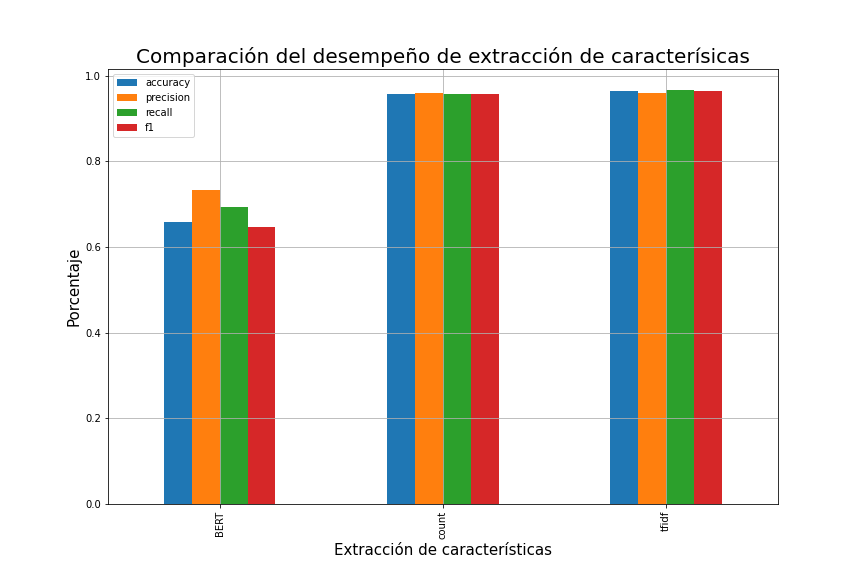
\includegraphics[width=\textwidth]{results/FakeNewsDetection/feature_extraction_comparison.png}
    \caption{Comparación de métodos de extracción de características}
    \label{fig:fake_news_feature_extraction}
\end{figure}

\subsubsection{Comparación por modelo de ML}
\begin{figure}
    \centering
    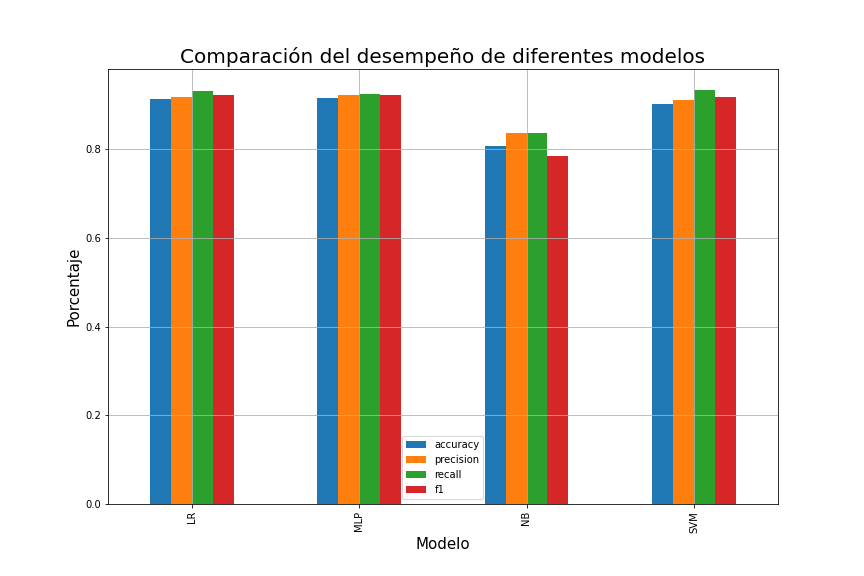
\includegraphics[width=\textwidth]{results/FakeNewsDetection/model_comparison.png}
    \caption{Comparación de modelos de ML}
    \label{fig:fake_news_models}
\end{figure}

\subsubsection{Comparación por idioma}
\begin{figure}
    \centering
    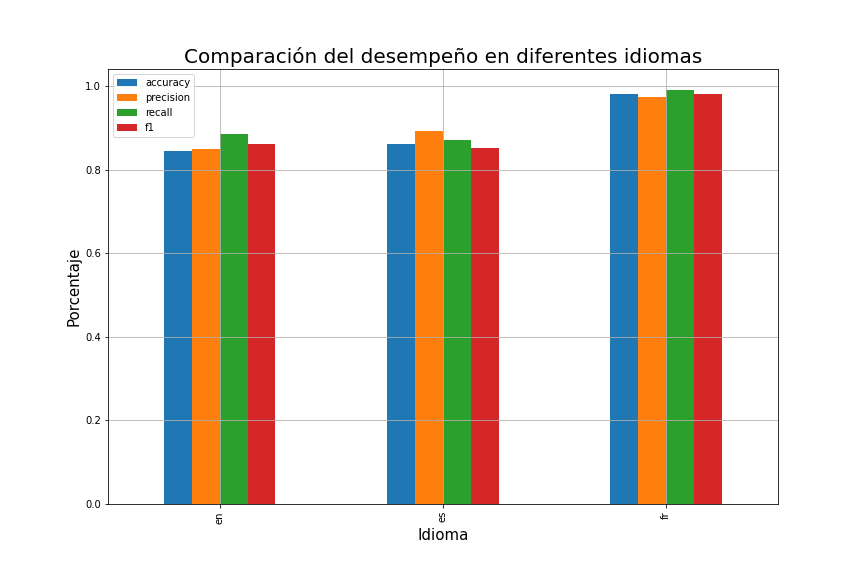
\includegraphics[width=\textwidth]{results/FakeNewsDetection/language_comparison.png}
    \caption{Comparación de idiomas}
    \label{fig:fake_news_languages}
\end{figure}

\subsection{Conclusiones}



\newpage
\bibliographystyle{unsrt}
\bibliography{biblist.bib}

\end{document}